\documentclass[11pt,a4paper]{article}
\usepackage[margin=0.75in]{geometry}
\usepackage{titlesec}
\usepackage{fontspec}
\usepackage{xcolor}
\usepackage{tikz}
\usepackage{enumitem}
\usepackage{fontawesome5}
\usepackage{varwidth}
\usepackage{hyperref}
\usepackage{multicol}
\usepackage{calc}
% Colors - Enhanced with a more tech-oriented palette
\definecolor{primaryblue}{RGB}{25, 118, 210}     % Deeper blue for main elements
\definecolor{secondaryblue}{RGB}{66, 165, 245}   % Lighter blue for secondary elements
\definecolor{dark}{RGB}{33, 33, 33}              % Nearly black for text
\definecolor{light}{RGB}{250, 250, 250}          % Off-white for backgrounds
\definecolor{highlight}{RGB}{255, 87, 34}        % Orange highlight for emphasis
\definecolor{projectbg}{RGB}{240, 245, 250}      % Light blue tint for project boxes
\definecolor{codegray}{RGB}{245, 245, 245}       % Light gray for code backgrounds
\definecolor{progressbg}{RGB}{230, 230, 230}     % Background for progress bars
\definecolor{progressfill}{RGB}{46, 204, 113}    % Green for progress indicators

% Fonts - Using a standard font to avoid font loading issues
\usepackage{lmodern}
% If you have Fira Sans installed, you can uncomment these lines:
\setmainfont[
     UprightFont = Fira Sans-Regular,
     BoldFont = Fira Sans-Bold,
     ItalicFont = Fira Sans-Italic,
     BoldItalicFont = Fira Sans-BoldItalic
]{Fira Sans}

% Title format
\titleformat{\section}
  {\LARGE\bfseries\color{primaryblue}}
  {}{0em}{}[\titlerule]
  
\titleformat{\subsection}
  {\Large\bfseries\color{dark}}
  {}{0em}{}

% Progress bar macro
\newcommand{\progressbar}[1]{%
  \begin{tikzpicture}
    \fill[progressbg] (0,0) rectangle (3,0.25);
    \fill[progressfill] (0,0) rectangle ({#1*3},0.25);
  \end{tikzpicture}%
}

% Custom commands for tech stack and progress indicators
\newcommand{\projecttitle}[1]{{\Large\bfseries\color{primaryblue} #1}}
\newcommand{\techstack}[1]{{\small\textbf{\color{dark}Tech Stack:} #1}}
\newcommand{\progress}[2]{%
  {\small\textbf{\color{dark}Progress:} #1 \hfill \progressbar{#2}}%
}

% Project box with Font Awesome icon - Fixed alignment
\newcommand{\projectbox}[4]{
    \noindent\begin{tikzpicture}
        \node[draw=secondaryblue, rounded corners=5pt, fill=projectbg, inner sep=10pt, text width=\linewidth-20pt] (box) {
            \begin{minipage}{\linewidth-40pt}
                \projecttitle{#1} \hfill {\color{primaryblue}\Large #2}
                \vspace{5pt}
                
                \textcolor{dark}{#3}
                \vspace{5pt}
                
                \techstack{#4}
            \end{minipage}
        };
    \end{tikzpicture}
}

% Project box with progress indicator - Fixed alignment
\newcommand{\projectboxprogress}[6]{
    \noindent\begin{tikzpicture}
        \node[draw=secondaryblue, rounded corners=5pt, fill=projectbg, inner sep=10pt, text width=\linewidth-20pt] (box) {
            \begin{minipage}{\linewidth-40pt}
                \projecttitle{#1} \hfill {\color{primaryblue}\Large #2}
                \vspace{5pt}
                
                \textcolor{dark}{#3}
                \vspace{5pt}
                
                \techstack{#4}
                \vspace{5pt}
                
                \progress{#5}{#6}
            \end{minipage}
        };
    \end{tikzpicture}
}

% Fixed skill level indicator - Fixed the numeric comparison issue
\newcommand{\skilllevel}[2]{
  \textbf{#1} \hfill 
  \begin{tikzpicture}[baseline]
    \foreach \x in {1,...,5} {
      \pgfmathparse{int(\x <= #2)}
      \ifnum\pgfmathresult=1
        \fill[primaryblue] (\x*0.6-0.5,0) circle (0.2);
      \else
        \draw[primaryblue] (\x*0.6-0.5,0) circle (0.2);
      \fi
    }
  \end{tikzpicture}\\
}

% Header and footer
\usepackage{fancyhdr}
\pagestyle{fancy}
\renewcommand{\headrulewidth}{0pt}
\fancyhead{}
\fancyfoot{}
\fancyfoot[C]{\thepage}

% Hyperlink styling
\hypersetup{
    colorlinks=true,
    linkcolor=primaryblue,
    urlcolor=primaryblue,
    citecolor=primaryblue
}

% Document
\begin{document}

% Title with tech-inspired background
\begin{tikzpicture}[remember picture, overlay]
    % Main background
    \fill[primaryblue] (current page.north west) rectangle ([yshift=-6cm]current page.north east);
    
    % Circuit pattern overlay
    \foreach \x in {0.5,1,...,20.5} {
      \foreach \y in {0.5,1,...,5.5} {
        \draw[white, opacity=0.1] (\x,\y) circle (0.05);
      }
    }
    \foreach \x in {1,3,...,19} {
      \foreach \y in {1,2,...,5} {
        \draw[white, opacity=0.1] (\x,\y) -- (\x+1,\y);
      }
    }
    \foreach \x in {2,4,...,20} {
      \foreach \y in {1,3,5} {
        \draw[white, opacity=0.1] (\x,\y) -- (\x,\y-0.5);
      }
    }
    
    % Title
    \node[text=white, anchor=center] at ([yshift=-3cm]current page.north) {
        \begin{varwidth}{\textwidth}
            \centering
            {\fontsize{32}{40}\selectfont \textbf{NOAM FAVIER}}\\[0.3cm]
            {\fontsize{18}{24}\selectfont SOFTWARE ENGINEERING PORTFOLIO}\\[0.2cm]
            {\fontsize{12}{16}\selectfont SYSTEMS PROGRAMMING • AI INTEGRATION • USER EXPERIENCE}
        \end{varwidth}
    };
\end{tikzpicture}

\vspace{6cm}

% Introduction
\begin{center}
\begin{minipage}{0.85\textwidth}
\centering
\textit{Innovative software engineer specializing in high-performance systems, AI integration, and intuitive user interfaces. Proficient in multiple programming paradigms with expertise in C++, Rust, Swift, and TypeScript.}
\end{minipage}
\end{center}

\vspace{1cm}

% Projects Section
\section{Featured Projects}

\subsection{System Utilities \& Monitoring}
\projectboxprogress{Sysmon-CLI}{\faTerminal}{A lightweight terminal-based system monitoring utility optimized for Mac \& Linux power users. Delivers real-time visualization of CPU utilization, memory allocation, disk I/O activity, and network statistics. Leverages efficient low-level system calls to ensure minimal performance impact while providing comprehensive system insights.}{C, POSIX syscalls, IOKit (macOS), procfs (Linux)}{Architecture planning completed. Initial implementation of CPU/memory tracking modules in progress.}{0.2}

\vspace{0.5cm}

\projectboxprogress{SysDash Ultra}{\faChartLine}{An advanced system monitoring dashboard that provides real-time visualization of CPU, RAM, process trees, GPU utilization, disk activity, and power metrics through an interactive interface. Features predictive performance analytics, hierarchical process visualization, and customizable threshold-based alerting.}{Rust, SwiftUI, sysctl (MacOS), WebGL, D3.js}{Backend core development underway with UI wireframing in progress.}{0.1}

\vspace{0.5cm}

\projectboxprogress{NetViz Pro}{\faProjectDiagram}{A cutting-edge network traffic analysis tool that renders inbound and outbound connections as an interactive 3D force-directed graph. Provides application-specific traffic monitoring, anomalous connection detection, and sophisticated filtering capabilities with stunning visual representations.}{Rust, SwiftUI, TypeScript, libpcap, BPF, WebGL, GraphQL}{Concept design and planning completed with UI prototype in active development.}{0.1}

\subsection{Developer Tools \& Productivity}
\projectboxprogress{Smart-Commit}{\faCode}{An AI-powered Git commit assistant that analyzes code changes to automatically generate contextually relevant commit messages. Ensures commits are descriptive, properly structured, and follow best practices through machine learning models trained on high-quality open-source repositories.}{C++, OpenAI API, libgit2, NLP (Natural Language Processing)}{Research and model training phase completed. Base commit message generation functionality implemented.}{0.3}

\vspace{0.5cm}

\projectboxprogress{CodeGrep}{\faSearch}{A high-performance, syntax-aware code search tool that understands programming language structures including function definitions, variable declarations, and partial queries. Utilizes abstract syntax tree parsing via Tree-sitter to deliver precise search results that respect code semantics rather than mere text matching.}{Rust, Tree-sitter, Regex, Fuzzy Matching Algorithms}{Implementation with advanced file indexing and search optimization in active development.}{0.4}

\vspace{0.5cm}

\projectboxprogress{Iris - AI Coding Assistant}{\faMicrochip}{A fully on-device AI-powered coding assistant for Neovim/VS Code that provides contextual code suggestions, intelligent refactoring recommendations, and interactive debugging assistance. Leverages locally-running language models to ensure privacy and eliminate cloud API dependencies.}{C++, Rust, Julia, SQLite, Redis, LLMs, Coqui TTS, Speech Recognition}{Neovim integration completed with AI reasoning module in active development.}{0.55}

\vspace{0.5cm}

\projectboxprogress{Neovim Config}{\faKeyboard}{A meticulously crafted Neovim configuration optimized for professional software development workflows. Features custom plugins, intuitive keybindings, intelligent code completion, and language-specific optimizations designed to maximize productivity and reduce context-switching.}{Lua, VimScript, Tree-sitter, LSP}{Ongoing refinement with regular updates based on workflow improvements.}{0.85}

\vspace{0.5cm}

\projectboxprogress{apple\_music.nvim}{\faMusic}{A Neovim plugin that integrates with Apple Music, allowing users to control playback directly from their editor. Features include play/pause, track skipping, and real-time display of the currently playing song. Designed for seamless music control without leaving the coding environment.}{Lua, AppleScript}{In development.}{0.8}

\vspace{0.5cm}

\projectboxprogress{2077.nvim}{\faPalette}{A Cyberpunk 2077-inspired Neovim theme designed with a futuristic neon aesthetic. Features optimized syntax highlighting, seamless lualine integration, and customizable UI elements. Provides an immersive and highly readable coding experience with vibrant color contrasts and ergonomic design considerations.}{Lua}{Fully completed and available for use.}{1.0}

\vspace{0.5cm}

\projectboxprogress{QueryCrust}{\faDatabase}{A sophisticated web-based database query management tool with an intuitive interface for optimizing and executing complex database operations. Built with modern web technologies and designed to simplify working with large and complex datasets through visual query building and optimization suggestions.}{React, TailwindCSS, Python, Flask, MySQL}{Completed and fully functional with all core features implemented.}{1.0}

\subsection{Content Management \& Organization}
\projectboxprogress{AutoSort}{\faFolderOpen}{A background file organization daemon that automatically categorizes and sorts files based on configurable rule sets. Supports intelligent sorting based on file type, naming patterns, metadata extraction, and content recognition through OCR processing.}{Go, fsnotify, YAML/JSON configuration, OCR processing (Tesseract)}{Core file detection and rule-based sorting logic implemented with OCR support in development.}{0.25}

\vspace{0.5cm}

\projectboxprogress{WorkTime}{\faClock}{An intelligent iOS application designed to automatically track productive hours through smart detection of active work sessions. Analyzes app usage patterns, device movement signatures, and Screen Time API data to generate comprehensive productivity analytics and trend visualizations.}{Swift, SwiftUI, CoreData, Screen Time API}{User interface design completed with data tracking integration in progress.}{0.3}

\subsection{Games \& Interactive Entertainment}
\projectboxprogress{ShadowedHunter}{\faGamepad}{A sophisticated Metroidvania-style game featuring intricate puzzles, advanced combat mechanics, and immersive storytelling. Built with a compelling narrative arc, character progression systems, and dynamic level design. Incorporates physics-based interactions, AI-driven enemy behaviors, and a comprehensive inventory management system.}{C\#, Unity, DOTween, A* Pathfinding}{Planning and development phase. Character animations and level layouts in active design.}{0.5}

\vspace{0.5cm}

\projectboxprogress{Pot Pot Golf}{\faGolfBall}{A physics-based 2D mini-golf simulation featuring realistic ball dynamics, variable terrain properties, and intelligent AI opponents. Players strategically control initial velocities and angles to navigate challenging courses with the fewest shots possible while contending with customizable friction and obstacle settings.}{Java, LWJGL, Box2D Physics}{Completed with full gameplay features, multiple courses, and AI opponent functionality.}{1.0}

\vspace{0.5cm}

\projectboxprogress{Chess Bot}{\faChess}{An intelligent chess engine implementing advanced heuristic-based decision making algorithms for move analysis and execution. Features positional evaluation, tactical calculation, and strategic planning capabilities that adapt to opponent play patterns through runtime optimization.}{Rust, minimax algorithm, alpha-beta pruning}{Core move generation and board representation implemented. Strategic evaluation algorithms in development.}{0.5}

\vspace{0.5cm}

\projectboxprogress{IDraughts Pro}{\faChessBoard}{A multiplayer Frisian Draughts game featuring real-time move validation, player-vs-player mode, and AI opponents. Implements a robust WebSocket server for seamless online play with intelligent move validation, disconnection handling, and game state recovery. AI opponents utilize Minimax and Deep Q-Network (DQN) algorithms for challenging gameplay.}{Rust, WebSockets, Minimax, DQN AI, Heroku}{Core game logic implemented with multiplayer server deployment in progress.}{0.9}

\subsection{Knowledge Management \& Learning}
\projectboxprogress{Thynkly}{\faLightbulb}{A comprehensive knowledge management platform combining note-taking, interactive mind mapping, and AI-driven flashcard generation. Designed to help users organize, visualize, and retain information efficiently. Features include real-time data synchronization, LaTeX support, collaborative editing, and AI-powered insights to enhance learning.}{[Tech Stack TBD]}{Application in active development, focusing on expanding features and refining user experience.}{0.2}

\subsection{Educational Technology}
\projectboxprogress{BitVoyager}{\faGraduationCap}{A browser-based gamified programming education platform where users complete interactive coding challenges in a simulated development environment. Features an XP-based progression system, skill trees, and a comprehensive curriculum covering multiple programming paradigms.}{TypeScript, WebAssembly, Python, Rust, xterm.js}{Interactive shell prototype completed with curriculum content in ongoing development.}{0.7}

\vspace{0.5cm}

\projectboxprogress{PyNexus}{\faIcon{mobile-alt}}{An intuitive iOS application designed to introduce beginners to Python programming through interactive exercises, visual feedback, and progressive challenges. Features step-by-step tutorials, real-time code execution, and achievement-based learning to keep users engaged and motivated.}{Swift, UIKit, Python interpreter integration}{Initial concept and design completed. Project currently on hold.}{0.2}

\section{Technical Expertise}

% Alternative skill representation without the problematic command
\begin{multicols}{2}
\subsection*{Languages}
\begin{itemize}[leftmargin=0pt, label={}]
    \item \textbf{C/C++} \hfill \tikz{\foreach \x in {1,...,5} {\fill[primaryblue] (\x*0.4-0.3,0) circle (0.15);}}
    \item \textbf{Rust} \hfill \tikz{\foreach \x in {1,...,4} {\fill[primaryblue] (\x*0.4-0.3,0) circle (0.15);} \draw[primaryblue] (5*0.4-0.3,0) circle (0.15);}
    \item \textbf{Swift} \hfill \tikz{\foreach \x in {1,...,5} {\fill[primaryblue] (\x*0.4-0.3,0) circle (0.15);}}
    \item \textbf{Go} \hfill \tikz{\foreach \x in {1,...,4} {\fill[primaryblue] (\x*0.4-0.3,0) circle (0.15);} \draw[primaryblue] (5*0.4-0.3,0) circle (0.15);}
    \item \textbf{TypeScript} \hfill \tikz{\foreach \x in {1,...,5} {\fill[primaryblue] (\x*0.4-0.3,0) circle (0.15);}}
    \item \textbf{Python} \hfill \tikz{\foreach \x in {1,...,4} {\fill[primaryblue] (\x*0.4-0.3,0) circle (0.15);} \draw[primaryblue] (5*0.4-0.3,0) circle (0.15);}
    \item \textbf{Julia} \hfill \tikz{\foreach \x in {1,...,3} {\fill[primaryblue] (\x*0.4-0.3,0) circle (0.15);} \foreach \x in {4,...,5} {\draw[primaryblue] (\x*0.4-0.3,0) circle (0.15);}}
\end{itemize}

\columnbreak

\subsection*{Frameworks \& Tools}
\begin{itemize}[leftmargin=0pt, label={}]
    \item \textbf{SwiftUI} \hfill \tikz{\foreach \x in {1,...,5} {\fill[primaryblue] (\x*0.4-0.3,0) circle (0.15);}}
    \item \textbf{Unity} \hfill \tikz{\foreach \x in {1,...,4} {\fill[primaryblue] (\x*0.4-0.3,0) circle (0.15);} \draw[primaryblue] (5*0.4-0.3,0) circle (0.15);}
    \item \textbf{WebGL} \hfill \tikz{\foreach \x in {1,...,3} {\fill[primaryblue] (\x*0.4-0.3,0) circle (0.15);} \foreach \x in {4,...,5} {\draw[primaryblue] (\x*0.4-0.3,0) circle (0.15);}}
    \item \textbf{React} \hfill \tikz{\foreach \x in {1,...,4} {\fill[primaryblue] (\x*0.4-0.3,0) circle (0.15);} \draw[primaryblue] (5*0.4-0.3,0) circle (0.15);}
    \item \textbf{Docker/K8s} \hfill \tikz{\foreach \x in {1,...,4} {\fill[primaryblue] (\x*0.4-0.3,0) circle (0.15);} \draw[primaryblue] (5*0.4-0.3,0) circle (0.15);}
    \item \textbf{Git/CI/CD} \hfill \tikz{\foreach \x in {1,...,5} {\fill[primaryblue] (\x*0.4-0.3,0) circle (0.15);}}
    \item \textbf{Neovim/VS Code} \hfill \tikz{\foreach \x in {1,...,5} {\fill[primaryblue] (\x*0.4-0.3,0) circle (0.15);}}
\end{itemize}
\end{multicols}

\vspace{0.5cm}

\noindent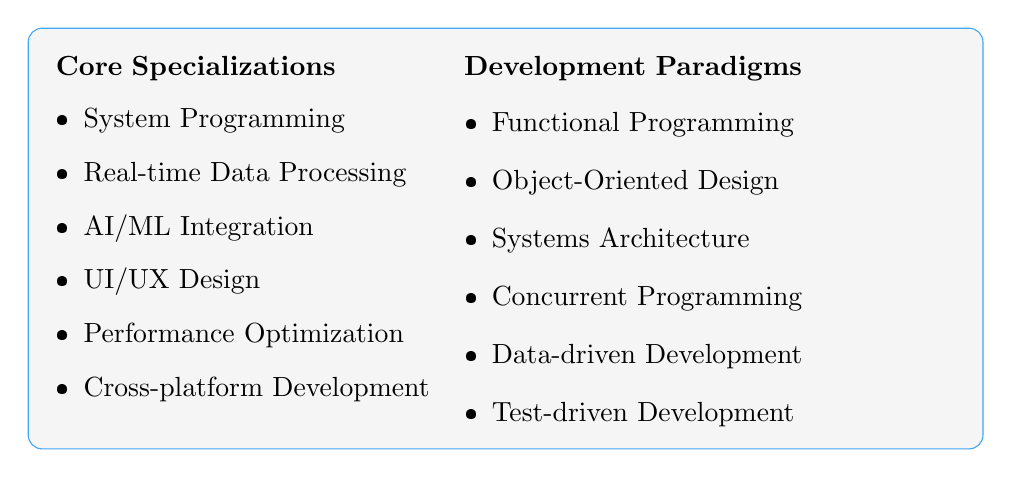
\begin{tikzpicture}
\node[draw=secondaryblue, rounded corners=5pt, fill=codegray, inner sep=10pt, text width=\linewidth-20pt] {
\begin{minipage}{\linewidth-40pt}
\begin{multicols}{2}
\textbf{Core Specializations}
\begin{itemize}[leftmargin=*]
    \item System Programming
    \item Real-time Data Processing
    \item AI/ML Integration
    \item UI/UX Design
    \item Performance Optimization
    \item Cross-platform Development
\end{itemize}

\columnbreak

\textbf{Development Paradigms}
\begin{itemize}[leftmargin=*]
    \item Functional Programming
    \item Object-Oriented Design
    \item Systems Architecture
    \item Concurrent Programming
    \item Data-driven Development
    \item Test-driven Development
\end{itemize}
\end{multicols}
\end{minipage}
};
\end{tikzpicture}

\vspace{1cm}

% Contact box with social icons
\begin{center}
\begin{tikzpicture}
    \node[draw=secondaryblue, rounded corners=5pt, fill=light, inner sep=12pt] {
        \begin{varwidth}{0.9\textwidth}
            \centering
            \small{For project demonstrations, code samples, and collaboration inquiries:}\\[0.2cm]
            \normalsize{
                \href{https://github.com/NoamFav}{\faGithub\ github.com/NoamFav} \hspace{1cm} 
                \href{https://noamfavier.dev}{\faGlobe\ noamfavier.dev} \hspace{1cm} 
                \href{mailto:noam.favier@icloud.com}{\faEnvelope\ noam.favier@icloud.com}
            }
        \end{varwidth}
    };
\end{tikzpicture}
\end{center}

\end{document}
